% Options for packages loaded elsewhere
\PassOptionsToPackage{unicode}{hyperref}
\PassOptionsToPackage{hyphens}{url}
\PassOptionsToPackage{dvipsnames,svgnames,x11names}{xcolor}
%
\documentclass[
  letterpaper,
  DIV=11,
  numbers=noendperiod]{scrartcl}

\usepackage{amsmath,amssymb}
\usepackage{lmodern}
\usepackage{iftex}
\ifPDFTeX
  \usepackage[T1]{fontenc}
  \usepackage[utf8]{inputenc}
  \usepackage{textcomp} % provide euro and other symbols
\else % if luatex or xetex
  \usepackage{unicode-math}
  \defaultfontfeatures{Scale=MatchLowercase}
  \defaultfontfeatures[\rmfamily]{Ligatures=TeX,Scale=1}
\fi
% Use upquote if available, for straight quotes in verbatim environments
\IfFileExists{upquote.sty}{\usepackage{upquote}}{}
\IfFileExists{microtype.sty}{% use microtype if available
  \usepackage[]{microtype}
  \UseMicrotypeSet[protrusion]{basicmath} % disable protrusion for tt fonts
}{}
\makeatletter
\@ifundefined{KOMAClassName}{% if non-KOMA class
  \IfFileExists{parskip.sty}{%
    \usepackage{parskip}
  }{% else
    \setlength{\parindent}{0pt}
    \setlength{\parskip}{6pt plus 2pt minus 1pt}}
}{% if KOMA class
  \KOMAoptions{parskip=half}}
\makeatother
\usepackage{xcolor}
\setlength{\emergencystretch}{3em} % prevent overfull lines
\setcounter{secnumdepth}{-\maxdimen} % remove section numbering
% Make \paragraph and \subparagraph free-standing
\ifx\paragraph\undefined\else
  \let\oldparagraph\paragraph
  \renewcommand{\paragraph}[1]{\oldparagraph{#1}\mbox{}}
\fi
\ifx\subparagraph\undefined\else
  \let\oldsubparagraph\subparagraph
  \renewcommand{\subparagraph}[1]{\oldsubparagraph{#1}\mbox{}}
\fi


\providecommand{\tightlist}{%
  \setlength{\itemsep}{0pt}\setlength{\parskip}{0pt}}\usepackage{longtable,booktabs,array}
\usepackage{calc} % for calculating minipage widths
% Correct order of tables after \paragraph or \subparagraph
\usepackage{etoolbox}
\makeatletter
\patchcmd\longtable{\par}{\if@noskipsec\mbox{}\fi\par}{}{}
\makeatother
% Allow footnotes in longtable head/foot
\IfFileExists{footnotehyper.sty}{\usepackage{footnotehyper}}{\usepackage{footnote}}
\makesavenoteenv{longtable}
\usepackage{graphicx}
\makeatletter
\def\maxwidth{\ifdim\Gin@nat@width>\linewidth\linewidth\else\Gin@nat@width\fi}
\def\maxheight{\ifdim\Gin@nat@height>\textheight\textheight\else\Gin@nat@height\fi}
\makeatother
% Scale images if necessary, so that they will not overflow the page
% margins by default, and it is still possible to overwrite the defaults
% using explicit options in \includegraphics[width, height, ...]{}
\setkeys{Gin}{width=\maxwidth,height=\maxheight,keepaspectratio}
% Set default figure placement to htbp
\makeatletter
\def\fps@figure{htbp}
\makeatother
\newlength{\cslhangindent}
\setlength{\cslhangindent}{1.5em}
\newlength{\csllabelwidth}
\setlength{\csllabelwidth}{3em}
\newlength{\cslentryspacingunit} % times entry-spacing
\setlength{\cslentryspacingunit}{\parskip}
\newenvironment{CSLReferences}[2] % #1 hanging-ident, #2 entry spacing
 {% don't indent paragraphs
  \setlength{\parindent}{0pt}
  % turn on hanging indent if param 1 is 1
  \ifodd #1
  \let\oldpar\par
  \def\par{\hangindent=\cslhangindent\oldpar}
  \fi
  % set entry spacing
  \setlength{\parskip}{#2\cslentryspacingunit}
 }%
 {}
\usepackage{calc}
\newcommand{\CSLBlock}[1]{#1\hfill\break}
\newcommand{\CSLLeftMargin}[1]{\parbox[t]{\csllabelwidth}{#1}}
\newcommand{\CSLRightInline}[1]{\parbox[t]{\linewidth - \csllabelwidth}{#1}\break}
\newcommand{\CSLIndent}[1]{\hspace{\cslhangindent}#1}

\KOMAoption{captions}{tableheading}
\makeatletter
\makeatother
\makeatletter
\makeatother
\makeatletter
\@ifpackageloaded{caption}{}{\usepackage{caption}}
\AtBeginDocument{%
\ifdefined\contentsname
  \renewcommand*\contentsname{Table of contents}
\else
  \newcommand\contentsname{Table of contents}
\fi
\ifdefined\listfigurename
  \renewcommand*\listfigurename{List of Figures}
\else
  \newcommand\listfigurename{List of Figures}
\fi
\ifdefined\listtablename
  \renewcommand*\listtablename{List of Tables}
\else
  \newcommand\listtablename{List of Tables}
\fi
\ifdefined\figurename
  \renewcommand*\figurename{Figure}
\else
  \newcommand\figurename{Figure}
\fi
\ifdefined\tablename
  \renewcommand*\tablename{Table}
\else
  \newcommand\tablename{Table}
\fi
}
\@ifpackageloaded{float}{}{\usepackage{float}}
\floatstyle{ruled}
\@ifundefined{c@chapter}{\newfloat{codelisting}{h}{lop}}{\newfloat{codelisting}{h}{lop}[chapter]}
\floatname{codelisting}{Listing}
\newcommand*\listoflistings{\listof{codelisting}{List of Listings}}
\makeatother
\makeatletter
\@ifpackageloaded{caption}{}{\usepackage{caption}}
\@ifpackageloaded{subcaption}{}{\usepackage{subcaption}}
\makeatother
\makeatletter
\@ifpackageloaded{tcolorbox}{}{\usepackage[many]{tcolorbox}}
\makeatother
\makeatletter
\@ifundefined{shadecolor}{\definecolor{shadecolor}{rgb}{.97, .97, .97}}
\makeatother
\makeatletter
\makeatother
\ifLuaTeX
  \usepackage{selnolig}  % disable illegal ligatures
\fi
\IfFileExists{bookmark.sty}{\usepackage{bookmark}}{\usepackage{hyperref}}
\IfFileExists{xurl.sty}{\usepackage{xurl}}{} % add URL line breaks if available
\urlstyle{same} % disable monospaced font for URLs
\hypersetup{
  pdftitle={Increase of GDP and Monetary Expansion},
  pdfauthor={Rae Zhang; Jenny Shen; Sarah Zhang},
  colorlinks=true,
  linkcolor={blue},
  filecolor={Maroon},
  citecolor={Blue},
  urlcolor={Blue},
  pdfcreator={LaTeX via pandoc}}

\title{Increase of GDP and Monetary Expansion\thanks{Code, data and
reproduction package are available at:
https://github.com/JunweiZhang130/Replication-for-The-real-effects-of-monetary-expansions-evidence-from-a-large-scale-history.git
and
https://www.socialsciencereproduction.org/reproductions/8d4a8d6c-9f9f-44dc-bd97-9c810ed677f6/index}}
\usepackage{etoolbox}
\makeatletter
\providecommand{\subtitle}[1]{% add subtitle to \maketitle
  \apptocmd{\@title}{\par {\large #1 \par}}{}{}
}
\makeatother
\subtitle{An Analysis of Potential Factors from 16th to 19th century}
\author{Rae Zhang \and Jenny Shen \and Sarah Zhang}
\date{22 February 2023}

\begin{document}
\maketitle
\begin{abstract}
This paper discusses the causal relationship between GDP growth and
monetary expansion from the 16th to the 19th century, with the intent to
identify the potential factors that contributed to economic growth
during this period. Using a historical analysis approach, the paper
examines multiple datasets including the nominal and real GDP of
different European countries, the production of precious metals in the
Americas, and the mint output of England that gave a glimpse to what
potentially stimulates economic growth. The findings suggest that
monetary injection played a significant role in increasing mint output
and driving GDP growth during this period. Additionally, the study
highlights the importance of monetary policies in promoting economic
development. Overall, this paper provides insights into the factors that
drove economic growth during a critical period in economic history.
\end{abstract}
\ifdefined\Shaded\renewenvironment{Shaded}{\begin{tcolorbox}[boxrule=0pt, frame hidden, enhanced, sharp corners, interior hidden, breakable, borderline west={3pt}{0pt}{shadecolor}]}{\end{tcolorbox}}\fi

\newpage

\hypertarget{introduction}{%
\section{1 Introduction}\label{introduction}}

During the early period, the discovery of massive deposits of precious
metals in the Americas resulted in monetary expansions to Europe's
supply. The finding of vast quantities of gold and silver in the New
World had a significant influence on the world economy's subsequent
history. The increase in the supply has reshaped the imports of consumer
goods across Europe, and one of the results is monetary expansions. The
effects of monetary policy have had major consequences, including
increased economic activity, higher investment rates, and enhanced
innovation. This paper explores the causal relationship of monetary
policy and production of metals, and its effect on the increase of GDP,
using historical data of the six European countries (Palma 2021).
Specifically, we will examine how the real GDP of European countries,
Gold and Silver production, and Mint output has impacted monetary
expansions. Some factors that we considered which influenced monetary
expansions on a variety of outcomes, including economic activity,
investment, and innovation.

We replicate the paper by Palma (Palma 2021) with a focus on the
following research questions:

\begin{itemize}
\tightlist
\item
  What is the trend in nominal GDP and real GDP over the period of 1500
  to 1800?
\item
  How does gold and silver share in America contribute to the trend of
  monetary expansion?
\item
  Why is mint output increasing from the period of 1500 to 1800 and how
  does it contribute to the monetary expansion?
\end{itemize}

The paper makes a significant contribution to our understanding of the
effects of monetary policy on the European economy, the importance of
historical analysis for understanding economic issues, and the relevance
of cross-country comparisons in economics. Specifically, it provides
evidence on the effects of large-scale monetary expansions in the 18th
century, which is a period where there was a widespread belief that
money supply increases would not have real effects on the economy. By
studying the historical analysis, we will have deeper insights into
current economic issues. Our goal is to organize the connections between
the trends of historical data in the 18th century. Explore how monetary
policy affects the real economy in Europe, especially England during the
period.

The analysis found that precious metals are one of the factors that
contributed to monetary expansion in the 18th century. When precious
metals, such as gold and silver were used as the basis for currency, it
caused an increase in demand within the country, or within international
trade, which led to monetary expansion. During the period of 1500 to
1800, production of precious metal increased which contributed to many
of the European country's GDP. In our reproduction of their paper, we
build on their ``monetary expansion'' explanation by expanding on the
relationship between Nominal GDP and Real GDP and the effect of precious
metals in the period of 1500 to 1800.

In this report, we will discuss the effects of monetary expansion on the
European economy. The first section of the report will be covering the
datasets we used for this analysis. The second section will be
addressing our findings from analyzing these data. Section 3 of the
report will expand on our findings and develop additional discussion on
the ethics and biases of the datasets. Finally, the last section of the
report will examine the weaknesses and potential of the overall paper.

\hypertarget{data}{%
\section{2 Data}\label{data}}

All figures in the paper are replicated from the original paper; The
replication material consist of two datasets: ``liquidity.dta'' and
``datadescriptive.dta''. ``liquidity.dta'' is the main datafile which is
used for the analysis and contains all variables used in the regression
analysis. ``datadescriptive.dta'' contains some additional variables
which is used for the descriptive figures.

The datasets for this report were obtained from the data section ``The
Real Effects of Monetary Expansion: Evidence from a Large-scale
Historical Experiment'' (Palma 2021), a paper from the Review of
Economic Studies. The data used by the paper was compiled by various
sources that spans a very long horizon (1531--1790), The most common
primary data sources for these studies are surviving account books of
the landed estates formerly belonging to local government and royal
administration, historical hospitals, prisons, charities, orphanages,
universities, and institutions of the church, particularly monasteries
and convents. GDP and prices come from the following sources: England
from Broadberry et al. (Broadberry et al. 2015), Holland from van Zanden
and van Leeuwen (Zanden and Leeuwen 2012), Spain from ¡lvarez-Nogal and
Prados de la Escosura (Alvarez-Nogal and Prados de la Escosura 2013),
Italy from Malanima (Malanima 2011), Portugal from Palma and Reis (2019)
and Germany from Pfister (Pfister 2020). When the original price level
was in silver it was transformed into monetary units using the
information given by Karaman et al. (Karaman, Pamuk, and
Yildirim-Karaman 2020). Englandís nominal mint output from
Challis(Challis 1992) and Palma's ``Reconstruction of money supply over
the long run: the case of England'' and ``Money and modernization in
early modern England''(Palma 2018). With regards to the innovation
component of gold arrivals, it is built using Costa et al. (Costa,
Rocha, and Sousa 2013) and Morineau(Morineau 2009) as explained in the
text. The data is mainly numeric, counting the number of the amount of
monetary activities in European countries.

The analysis will be carried out using the statistical programming
language \texttt{R} (R Core Team 2022), using the \texttt{haven}
(Wickham, Miller, and Smith 2022) and \texttt{tidyverse} (Wickham et al.
2019) packages. All figures in the report are generated using
\texttt{ggplot2} (Wickham 2016).

\newpage

\hypertarget{results}{%
\section{3 Results}\label{results}}

\hypertarget{the-real-and-nominal-gdp-over-the-period-of-1500-to-1800}{%
\subsection{The Real and Nominal GDP over the Period of 1500 to
1800}\label{the-real-and-nominal-gdp-over-the-period-of-1500-to-1800}}

\begin{figure}

{\centering 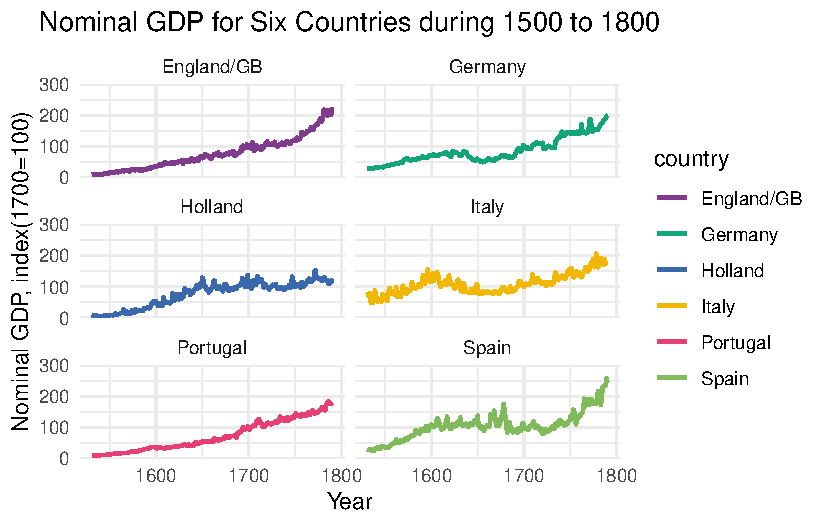
\includegraphics{paper_files/figure-pdf/fig-nominalgdp-1.pdf}

}

\caption{\label{fig-nominalgdp}shows the nominal GDP of six countries
from 1500 to 1800. *Nominal gross domestic product (GDP) is GDP given in
current prices, without adjustment for inflation ({``Nominal {Gross}
{Domestic} {Product} {GDP}''} 2023)}

\end{figure}

In Figure~\ref{fig-nominalgdp}, The vertical axis shows the Nominal
Gross Domestic Product (GDP) index (normalized to 1700=100), and the
horizontal axis shows the year. Each graph represents one of the six
countries, and the colours determine each country. The plot is intended
to show the differences in the economic development of different
countries over time.The impact of precious metals on GDP (Gross Domestic
Product) can vary depending on several factors such as the type of
metal, the production levels, and the overall demand for the metal. The
data shows that there were significant differences in the level of
economic development between these countries during this time period,
with the United Kingdom and the Netherlands having the highest levels of
nominal GDP, and Spain and Portugal having the lowest levels. \newpage

\begin{figure}

{\centering 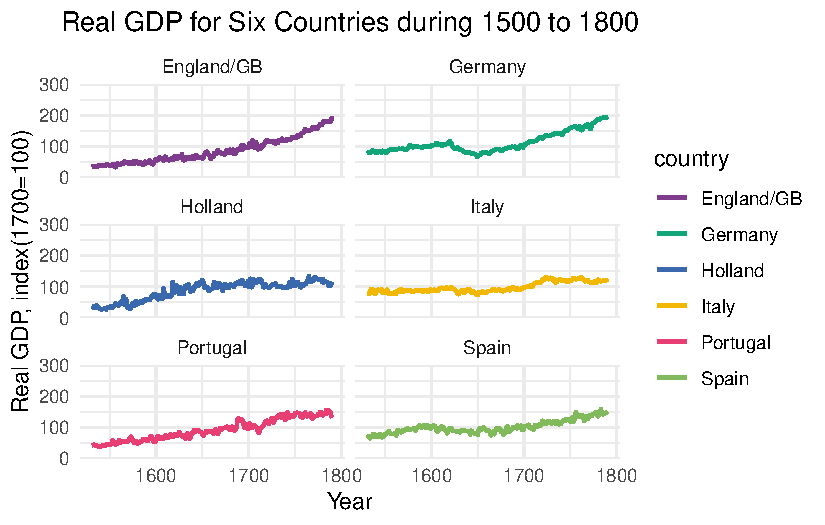
\includegraphics{paper_files/figure-pdf/fig-realgdp-1.pdf}

}

\caption{\label{fig-realgdp}displays the Real GDP of six European
countries over the period of 1500 - 1800, *Real gross domestic product
(GDP) is GDP given in constant prices and refers to the volume level of
GDP ({``{Real GDP forecast (indicator)}''} 2023).}

\end{figure}

Figure~\ref{fig-realgdp} has a similar plot with
Figure~\ref{fig-nominalgdp}, the vertical axis shows the Real GDP index
(normalized to 1700=100), and the horizontal axis shows the year. the
response of output to a monetary expansion in the six countries from
1500 to 1800. The results indicate that the response of output varied
widely between countries, with some countries experiencing a large
increase in output in response to monetary expansion (e.g., the
Netherlands), while others experienced little to no response (e.g.,
Spain). Additionally, the response of output to monetary expansion
changed over time, with some countries experiencing a greater response
in the earlier period of the study (e.g., Germany) and others
experiencing a greater response in the later period (e.g., the United
Kingdom).

Overall, these figures illustrate the heterogeneity of economic
development across countries and the diversity of responses to monetary
policy, highlighting the importance of country-specific factors in
determining the impact of monetary policy.

\begin{figure}

{\centering 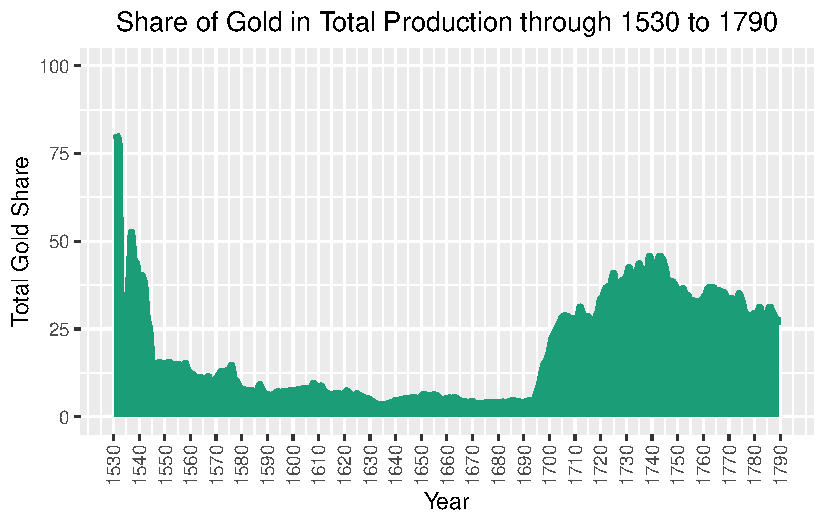
\includegraphics{paper_files/figure-pdf/fig-goldshare-1.pdf}

}

\caption{\label{fig-goldshare}Total Goldshare through 1530 to 1790}

\end{figure}

\newpage

As shown in the graph(Figure~\ref{fig-goldshare}), the mining of gold
and silver culminated in the 1530s from the occurrence of Mexican and
Peruvian acquisitions (Davenport 2012). The Mexican and Peruvian
conquests resulted in an outstanding increment in the production of
precious metals under Spanish colonisation. However, the annual
production of precious metals decreased significantly in the late
sixteenth century all the way through the late seventeenth century due
to factors such as shipwrecks, rivalries, and the lacking resources of
gold (Woodward and Bushnell, n.d.). It was not until the 1700s the share
of gold and silver surges again with the new streams of Brazilian and
Mexican production of precious metals (Guerra 2004).

It is important to note that the early monetary system was a commodity
money system and there were no central banks but only one form of
monetary policy, which is the control of the rate at which private
agents could transform precious metals into currency. Hence, the
production of precious metals mattered for how much new coin was minted.

\begin{figure}

{\centering 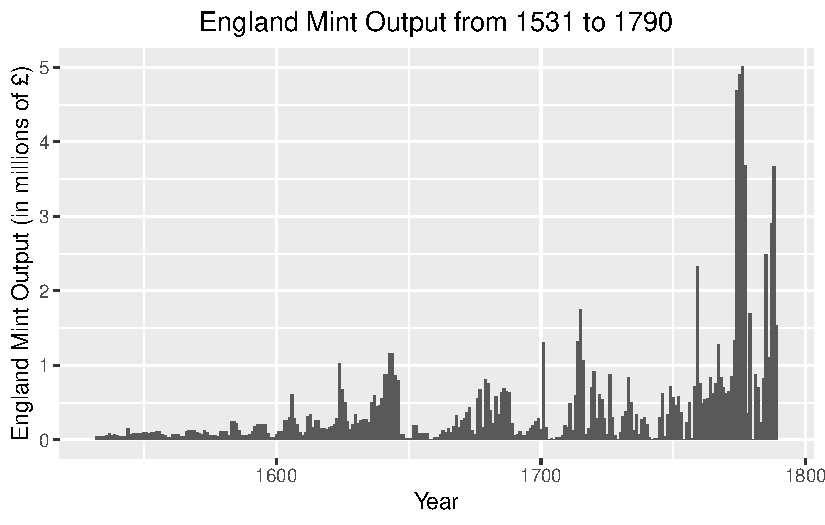
\includegraphics{paper_files/figure-pdf/fig-mintoutput-1.pdf}

}

\caption{\label{fig-mintoutput}England Mint Output from 1531 to 1790}

\end{figure}

\hypertarget{disucussion}{%
\section{4 Disucussion}\label{disucussion}}

\hypertarget{cohort-effect-in-european-countries}{%
\subsection{4.1 Cohort Effect in European
Countries}\label{cohort-effect-in-european-countries}}

The paper examines the impact of monetary expansions on the GDP changes
in six European countries from the 16th to 19th century. During 1800,
with cheaper transportation and mass production, goods no longer had to
be made near to where they were consumed, which encouraged monetary
expansion.the paper provides strong evidence that monetary expansions
can have significant real effects on economic activity. This is
demonstrated through the analysis of the historical experiment where six
European countries experienced large-scale monetary expansions in the
18th century. The paper shows that monetary expansions were associated
with an increase in output, which in turn led to an increase in nominal
GDP in the 18th and 19th centuries. The link between monetary
expansions, mint output, and GDP is intuitive. When the money supply
increases, individuals and firms have more money to spend, which leads
to an increase in demand for goods and services. This, in turn,
stimulates production and leads to an increase in output. With a higher
output, the economy as a whole is able to produce more, which leads to
an increase in both nominal and real GDP.

\hypertarget{a-case-of-monetary-expansion-englands-mint-output}{%
\subsection{4.2 A Case of Monetary Expansion: England's Mint
Output}\label{a-case-of-monetary-expansion-englands-mint-output}}

Figure~\ref{fig-mintoutput} illustrates the English nominal mint output
from 1531 - 1790 period. Mint output refers to the amount of new
currency that is produced over the period of time, which can be measured
using the quantity of the coins that are produced. The Mint output was a
steady decrease in the issue of gold coins and sharper increase in the
production of silver coins. This is primarily caused by the proportion
of silver to gold coins. The mint output was relatively low in the
fourteenth century, but as the picture indicates, it surged from the
sixteenth century onward. During the 16th century, the world gold-silver
ratio grew, as world stocks increased, the less precious metal continued
to depreciate.

In the 18th century, England adopted the gold standard, which meant that
the value of coins was tied to the value of gold. This led to an
increase in the production of gold coins, which caused the output of the
mint to fluctuate. This also explains the peaks during 1770-1780, as the
mint output reached 5 million pounds. The mint output tripled in late
1700, which could be caused by several factors such as the growth of
international trade. As England's economy grew and trade with other
countries increased, there was a greater demand for currency to
facilitate commerce (Gould 1952). This supports the evidence that
increase in American precious metals inevitably results in growth in
European money supply, particularly for second-wave receivers like
England, who obtained it mostly through trade with Spain and Portugal.

As seen in Figure~\ref{fig-nominalgdp} and Figure~\ref{fig-realgdp}, the
trend of mint output is linked to the trend of GDP, which can fluctuate
and vary based on the economic activity of the period. While mint output
of precious metals can be linked to GDP, it is worth noting that the
output is not always increasing and can be volatile. This volatility is
caused by fluctuations in the market, which are impacted by supply and
demand within the country and in international trade. These fluctuations
can lead to price increases or decreases and can be reflected in exports
and imports of precious metals, which can, in turn, affect the
profitability of mining companies and ultimately impact GDP.

\hypertarget{how-does-mint-output-and-monetary-expansion-contribute-to-todays-economy}{%
\subsection{4.3 How Does Mint Output and Monetary Expansion Contribute
to Today's
Economy?}\label{how-does-mint-output-and-monetary-expansion-contribute-to-todays-economy}}

Mint output impacts today's economy in several ways including
facilitating transactions, generating revenue, supporting financial
stability, and promoting national identity. In daily life, increasing
mint output makes it easier and more convenient for people to purchase
goods and services, pay bills, and conduct financial transactions. While
the process of producing new currencies and coins helps generate revenue
for the government, which can then be used to fund public services and
infrastructures. A reliable and consistent mint output could also make
certain an adequate amount of currency in circulation, ensuring there
will not be disruptions in the financial system. Furthermore, currencies
and coins often feature national symbols and images that promote a
country's cultural identity and heritage, creating a positive and
lasting effect on tourism and international trade.

On the other hand, the effects of monetary expansion on economic
activities are more complex. Monetary expansion can affect the economy
through changes in interest rates, money supply, exchange rates, and
GDP. The decrease in interest rates could stimulate economic growth by
encouraging individuals and businesses to borrow more money in order to
spend and make investments. However, it can also lead to inflation when
the amount of mint output becomes greater than the supply of goods and
services in the economy. Additionally, monetary expansion can depreciate
the value of the currency since a lower interest rate often makes a
country's currency less attractive to investors from a foreign country.
And from the findings of this paper, monetary injections are proven to
be the cause of increase in both nominal and real GDP of different
countries. Overall, monetary expansion can have positive effects such as
stimulating the growth of the economy, but it can also instigate
negative effects such as inflation if not managed properly.

\hypertarget{bias-and-ethical-concerns}{%
\subsection{4.4 Bias and Ethical
Concerns}\label{bias-and-ethical-concerns}}

The paper by Palma (Palma 2021) relies on a large dataset of economic
indicators and variables, which is mostly made up of long-term
historical data. The use of such data introduces several potential
sources of bias that could impact the statistical analysis and
interpretation of the results. One potential source of bias is selection
bias. Firstly, the paper focuses on European countries and may not be
generalizable to other regions. This could introduce sampling bias
because the findings may not generalize to other contexts or time
periods. Economic and institutional conditions in Europe during the
historical period analyzed in the paper were unique and different from
those in other regions and time periods. Therefore, it is possible that
the results may not be applicable to other economies or time periods.

Furthermore, the use of historical data can introduce additional biases,
such as measurement error, missing data, and differences in data quality
across time and regions. This can potentially affect the accuracy and
reliability of the results, as well as limit the generalizability of the
findings. Additionally, the availability and quality of data may have
been influenced by political and economic factors, which can further
affect the validity and reliability of the results.

\hypertarget{weakness}{%
\section{5 Weakness}\label{weakness}}

In the reproduction process, we translate the original STATA language
into R, meanwhile, we updated the profile name to make it better
organized in the folder. However, the paper still has many weaknesses.
For example, the information Palma provided in the package was
incomplete. Additionally, considering source was collected from local
governments and account books, and the data was from an old range of
period. Errors in the dataset can occur. Due to this, the conclusion
that we draw from this graph are likely not accurate to reflect the
overall trend of GDP. Our research question focused on the trend of GDP
over the period of 1500 to 1800, and only focusing on the precious
metal. Yet our conclusion was drawn from the six countries and does not
reflect the world.

\newpage

\hypertarget{references}{%
\section*{References}\label{references}}
\addcontentsline{toc}{section}{References}

\hypertarget{refs}{}
\begin{CSLReferences}{1}{0}
\leavevmode\vadjust pre{\hypertarget{ref-AlvarezNogal2013}{}}%
Alvarez-Nogal, Carlos, and Leandro Prados de la Escosura. 2013. {``The
Rise and Fall of Spain (1270-1850).''} \emph{The Economic History
Review} 66 (1): 1--37.

\leavevmode\vadjust pre{\hypertarget{ref-Broadberry2015}{}}%
Broadberry, Stephen, Bruce Campbell, Alexander Klein, Mark Overton, and
Bas van Leeuwen. 2015. \emph{British Economic Growth, 1270-1870}.
Cambridge University Press.

\leavevmode\vadjust pre{\hypertarget{ref-Challis1992}{}}%
Challis, C. 1992. {``Lord Hastings to the Great Silver Recoinage
1464-1699.''} In \emph{New History of the Royal Mint}, edited by C.
Challis. Cambridge University Press.

\leavevmode\vadjust pre{\hypertarget{ref-Costa2013}{}}%
Costa, L. F., M. M. Rocha, and R. Sousa. 2013. \emph{O Ouro Do Brasil}.
Imprensa Nacional-Casa da Moeda.

\leavevmode\vadjust pre{\hypertarget{ref-davenport_2012}{}}%
Davenport, Jade. 2012. {``Spanish Conquistadors and the Looting of
Mexican and Peruvian Golden Treasure.''} \emph{Mining Weekly}.
\url{https://www.miningweekly.com/article/spanish-conquistadors-and-the-looting-of-mexican-and-peruvian-golden-treasure-2012-09-07}.

\leavevmode\vadjust pre{\hypertarget{ref-Gould}{}}%
Gould, J. D. 1952. {``The Royal Mint in the Early Seventeenth
Century.''} \emph{The Economic History Review} 5 (2): 240--48.
\url{http://www.jstor.org/stable/2591058}.

\leavevmode\vadjust pre{\hypertarget{ref-GUERRA20041225}{}}%
Guerra, M. F. 2004. {``The Circulation of South American Precious Metals
in Brazil at the End of the 17th Century.''} \emph{Journal of
Archaeological Science} 31 (9): 1225--36.
https://doi.org/\url{https://doi.org/10.1016/j.jas.2004.03.018}.

\leavevmode\vadjust pre{\hypertarget{ref-Karaman2020}{}}%
Karaman, K. K., S. Pamuk, and S. Yildirim-Karaman. 2020. {``Money and
Monetary Stability in Europe, 1300--1914.''} \emph{Journal of Monetary
Economics} 115: 279--300.

\leavevmode\vadjust pre{\hypertarget{ref-Malanima2011}{}}%
Malanima, Paolo. 2011. {``The Long Decline of a Leading Economy: GDP in
Central and Northern Italy, 1300-1913.''} \emph{European Review of
Economic History} 15: 169--219.

\leavevmode\vadjust pre{\hypertarget{ref-Morineau2009}{}}%
Morineau, Michel. 2009. \emph{Incroyables Gazettes Et Fabuleux MÈtaux:
Les Retours Des TrÈsors AmÈricains díAprËs Les Gazettes Hollandaises
(XVI-XVII SiËcles)}. Cambridge University Press.

\leavevmode\vadjust pre{\hypertarget{ref-oecd_nominal_gdp_forecast}{}}%
{``Nominal {Gross} {Domestic} {Product} {GDP}.''} 2023. OECD.
\url{https://data.oecd.org/gdp/nominal-gdp-forecast.htm/\#:/~:text=Nominal/\%20gross/\%20domestic/\%20product/\%20(GDP,in/\%20the/\%20current/\%20reporting/\%20period}.

\leavevmode\vadjust pre{\hypertarget{ref-Palma2018b}{}}%
Palma, Nuno. 2018. {``Money and Modernization in Early Modern
England.''} \emph{Financial History Review} 25 (3): 231--61.

\leavevmode\vadjust pre{\hypertarget{ref-PalmaRealEffect}{}}%
---------. 2021. {``{The Real Effects of Monetary Expansions: Evidence
from a Large-scale Historical Experiment}.''} \emph{The Review of
Economic Studies} 89 (3): 1593--1627.
\url{https://doi.org/10.1093/restud/rdab042}.

\leavevmode\vadjust pre{\hypertarget{ref-Pfister2020}{}}%
Pfister, Ulrich. 2020. {``Economic Growth in Germany, 1500-1800.''}

\leavevmode\vadjust pre{\hypertarget{ref-citeR}{}}%
R Core Team. 2022. \emph{R: A Language and Environment for Statistical
Computing}. Vienna, Austria: R Foundation for Statistical Computing.
\url{https://www.R-project.org/}.

\leavevmode\vadjust pre{\hypertarget{ref-oecd_real_gdp_forecast}{}}%
{``{Real GDP forecast (indicator)}.''} 2023. OECD.
\url{https://data.oecd.org/gdp/real-gdp-forecast.htm\#:~:text=Real\%20gross\%20domestic\%20product\%20(GDP,terms\%20of\%20a\%20base\%20period}.

\leavevmode\vadjust pre{\hypertarget{ref-citeggplot2}{}}%
Wickham, Hadley. 2016. \emph{Ggplot2: Elegant Graphics for Data
Analysis}. Springer-Verlag New York.
\url{https://ggplot2.tidyverse.org}.

\leavevmode\vadjust pre{\hypertarget{ref-citetidyverse}{}}%
Wickham, Hadley, Mara Averick, Jennifer Bryan, Winston Chang, Lucy
D'Agostino McGowan, Romain François, Garrett Grolemund, et al. 2019.
{``Welcome to the {tidyverse}.''} \emph{Journal of Open Source Software}
4 (43): 1686. \url{https://doi.org/10.21105/joss.01686}.

\leavevmode\vadjust pre{\hypertarget{ref-citehaven}{}}%
Wickham, Hadley, Evan Miller, and Danny Smith. 2022. \emph{Haven: Import
and Export 'SPSS', 'Stata' and 'SAS' Files}.
\url{https://CRAN.R-project.org/package=haven}.

\leavevmode\vadjust pre{\hypertarget{ref-woodward_bushnell}{}}%
Woodward, Ralph Lee, and David Bushnell. n.d. {``The Habsburg Period
(1524--1700).''} \emph{Encyclopædia Britannica}. Encyclopædia
Britannica, inc.
\url{https://www.britannica.com/place/Central-America/The-Habsburg-period-1524-1700}.

\leavevmode\vadjust pre{\hypertarget{ref-vanZanden2012}{}}%
Zanden, J. L. van, and B. van Leeuwen. 2012. {``Persistent but Not
Consistent: The Growth of National Income in Holland 1347-1807.''}
\emph{Explorations in Economic History} 49: 119ñ130.

\end{CSLReferences}



\end{document}
